\documentclass[a4j,12pt,]{jarticle}
 \usepackage{float}
 \usepackage{siunitx} %%SI単位系用
 \usepackage{amssymb, amsmath}
 \usepackage{ascmac,here,txfonts}
 \usepackage{hyperref}
 \usepackage{listings}
 \usepackage{pxjahyper}
 \usepackage[dvipdfmx]{graphicx}
 \usepackage{amssymb, amsmath}
  \usepackage{listings}
  \usepackage[dvipdfmx]{color}
 
 \lstset{
   language={Python},
   basicstyle={\ttfamily},
   identifierstyle={\small},
   commentstyle={\small\itshape},
   keywordstyle={\small\bfseries},
   ndkeywordstyle={\small},
   stringstyle={\small\ttfamily},
   frame={single},
   breaklines=true,
   columns=[l]{fullflexible},
   numbers=left,
   xrightmargin=0zw,
   xleftmargin=3zw,
   numberstyle={\scriptsize},
   stepnumber=1,
   numbersep=1zw,
   lineskip=-0.5ex,
 }
\begin{document}

{\noindent\small  \hfill\today}
\begin{center}
  {\Large まつやまRe・再来館設置システムの実測データと理論データの時刻修正に関する研究の中間報告}
\end{center}
\begin{flushright}
  祖父江匠真 \\
\end{flushright}

\section{概要}
松山市教育委員会によって小学校などに設置されている太陽発電計測システムのPCは, まつやまRe・再来館に設置されているものを除くと, インターネットに接続されていないオフライン環境で計測が行われている. このため, PCの内部時計が経過時間とともにずれており, 実測データのタイムスタンプが不正な値になっている.

そこで, タイムスタンプの修正を行うために, 実測データと, 太陽光発電シミュレーターにより生成された理論データとの, 相互相関関数を用いた時刻合わせプログラムの実装を行っている.

その時刻合わせプログラムを実行した際に, 結果として得られるずれ時間の推定結果が正しいことを確認するため, タイムスタンプが正確な実測データを用いてずれ時間の推定結果が0秒となることを確認する作業を現在行っている.

まつやまRe・再来館に設置されている計測システムはインターネットに接続されており, さらにシステムを実行しているマイコンを24時間ごとに再起動しているため, マイコン内部の時計は常にインターネット時刻に同期されており, 計測データのタイムスタンプは正確である.

本報告では, まつやまRe・再来館の実測データを入力として時刻合わせプログラムを実行した際の, ずれ時間の推定結果について述べる.

\section{相互相関とは}
相互相関は, 2つの信号の類似性を測定するために用いられる手法の一つである. 相互相関を用いることで, 2つの信号の類似度を示す数値を算出し, 信号間の関係を調査することができる. 相互相関値が高ければ高いほど, 2つの信号は互いに類似していると言える.

相互相関を用いた信号間のずれの検出方法は以下の手順で行われる\cite{1}.

\begin{enumerate}
  \item 2つの異なる雑音信号(信号Aおよび信号Bとする)を用意する. ただしこれらの信号の雑音が大きい時間は同じ長さである.
  \item 信号Aと信号Bをずらしながら重ね合わせる. このずらしの大きさを「ラグ時間」と称する. ラグ時間が0である場合, 信号Aと信号Bは完全に一致する状態である. ラグ時間が正である場合, 信号Bは信号Aより遅れていることを示し, ラグ時間が負である場合はその逆である.
  \item それぞれのラグ時間において, 信号Aと信号Bが重なる部分の積の和(内積)を算出する. これを相互相関と呼ぶ.
  \item それぞれのラグ時間ごとに相互相関を計算し, 相互相関が最大となる際のラグ時間を特定する. この際に得られたラグ時間は, 信号Aと信号Bのずれ時間を示している.
\end{enumerate}

例として, 図 \ref{p1}に示す2つの信号sig1, sig2に対して相互相関を計算した場合, sig2を右に800秒スライドさせた際に相互相関が最大となるため, これらのラグ時間は800秒であると計算される. 信号fitはsig2を800秒分右へスライドさせたものとsig1を重ねてプロットしたものであり, 相互相関によってずれ時間が正しく推定出来ていることが分かる.

\begin{figure}[H]
  \begin{center}
    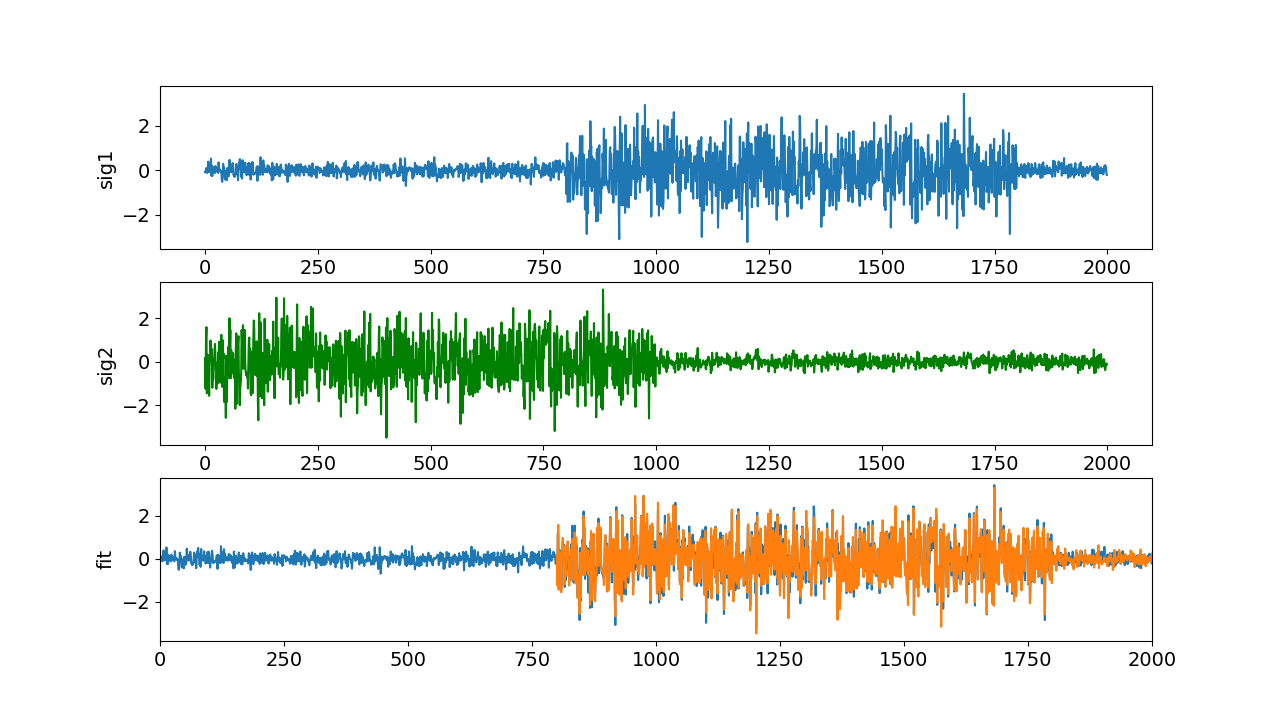
\includegraphics[width=160mm]{corr_sample.png}
    \caption{相互相関に使用した信号とずれ時間分スライドさせて重ねたもの}
    \label{p1}
  \end{center}
\end{figure}

\section{理論データのシミュレーション方法について}
理論データのシミュレーションは, 太陽光発電システムのシミュレーションを行うためのPythonライブラリであるPvlibを用いて行う\cite{2}.

Pvlibを用いることで緯度, 経度, 標高, タイムゾーン, 日時などを入力として, 快晴時の地表に到達する日射量を推定することができる.

例として, 2022年4月8日に計測された実測データを取り上げ, それに対応する理論データをPvlibで計算して合わせてプロットすることで, Pvlibの予測精度がどの程度のものか視覚的に説明する.

% 晴天の日における日射量の推定は, 以下の手順で進める. 

% \begin{enumerate}
% \item \textbf{位置情報の設定}: まず, 緯度, 経度, 標高, タイムゾーンなどを指定し, \\\texttt{pvlib.location.Location}オブジェクトを生成する. このオブジェクトは, 太陽位置や日射量の計算に使用される. 
% \item \textbf{日時データの準備}: 推定対象の日時範囲を指定し, 対応する表データを作成する. 
% \item \textbf{太陽位置の計算}: \texttt{pvlib.solarposition.get\_solarposition}関数を用いて, 指定された位置情報および日時データを基に, 太陽の高度角と方位角を計算する. 
% \item \textbf{大気透過率の計算}: \texttt{pvlib.clearsky.ineichen}関数を使用し, 大気透過率を計算する. この関数は, 指定された位置情報と太陽位置に基づいて, 大気の透過率を推定し, 全天日射量, 直達日射量, 拡散日射量を計算する. 
% \item \textbf{地表での日射量の推定}: 最後に, \texttt{pvlib.irradiance.get\_total\_irradiance}関数を用いて, 地表での日射量を推定する. この関数は, 太陽位置, 大気透過率, 入射角などの情報に基づいて, 地表での直達日射量, 拡散日射量, 反射日射量を計算する. 
% \end{enumerate}

% これらの手順に従って, 晴天の日における地表での日射量を推定することができる. 得られた日射量データは, 実測データとの比較に利用される. 

図 \ref{p2}に示すのは2022年4月8日に松山Re・再来館で計測された実測データである.

\begin{figure}[H]
  \begin{center}
    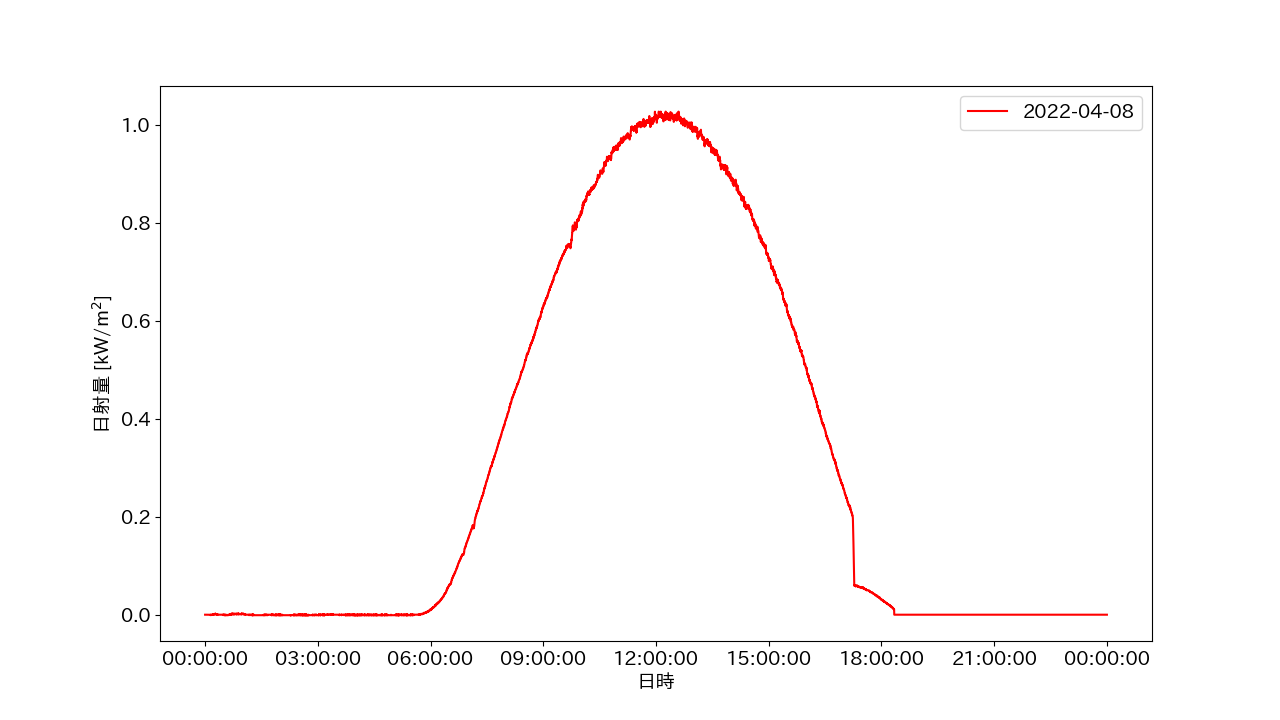
\includegraphics[width=160mm]{real.png}
    \caption{2022年4月8日の実測データ}
    \label{p2}
  \end{center}
\end{figure}

図 \ref{p2}の実測データのタイムスタンプ列をPvlibに入力し, シミュレーションした結果を図 \ref{p3}に示す.

\begin{figure}[H]
  \begin{center}
    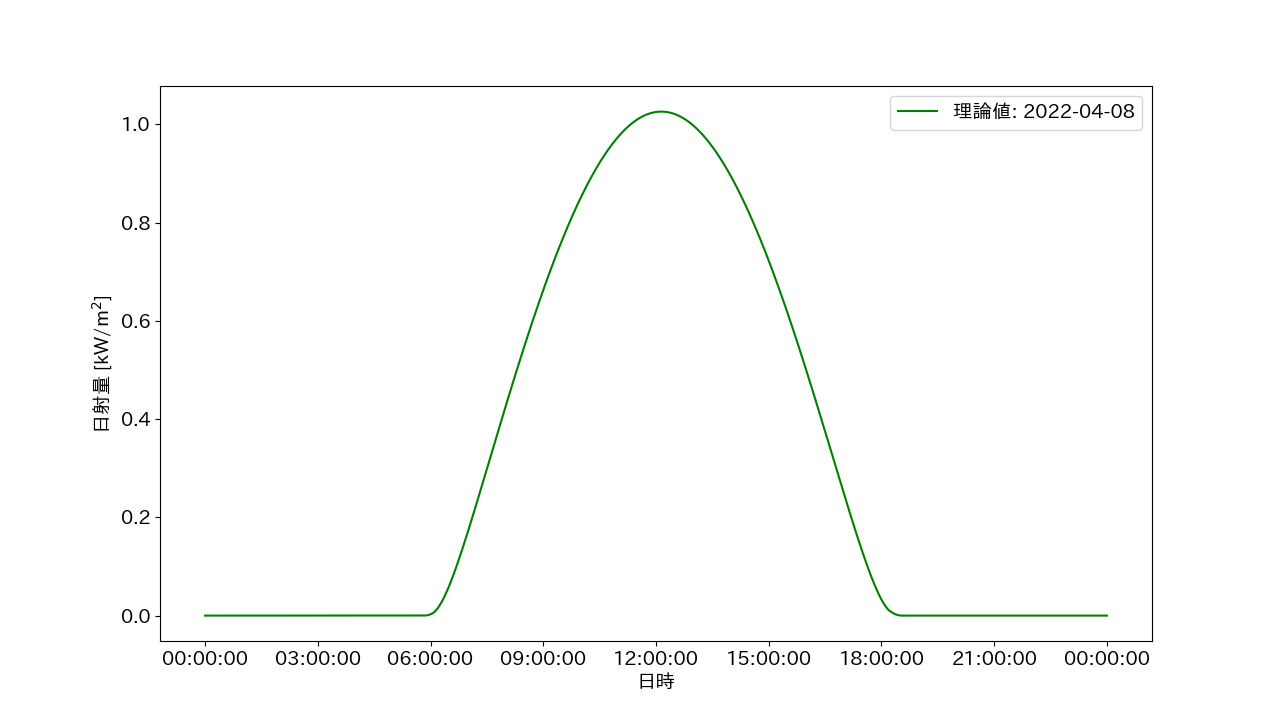
\includegraphics[width=160mm]{theoretical.png}
    \caption{2022年4月8日の実測データに対応する理論データ}
    \label{p3}
  \end{center}
\end{figure}

実測データと理論データを合わせてプロットしたものを, 図 \ref{p4}に示す.

\begin{figure}[H]
  \begin{center}
    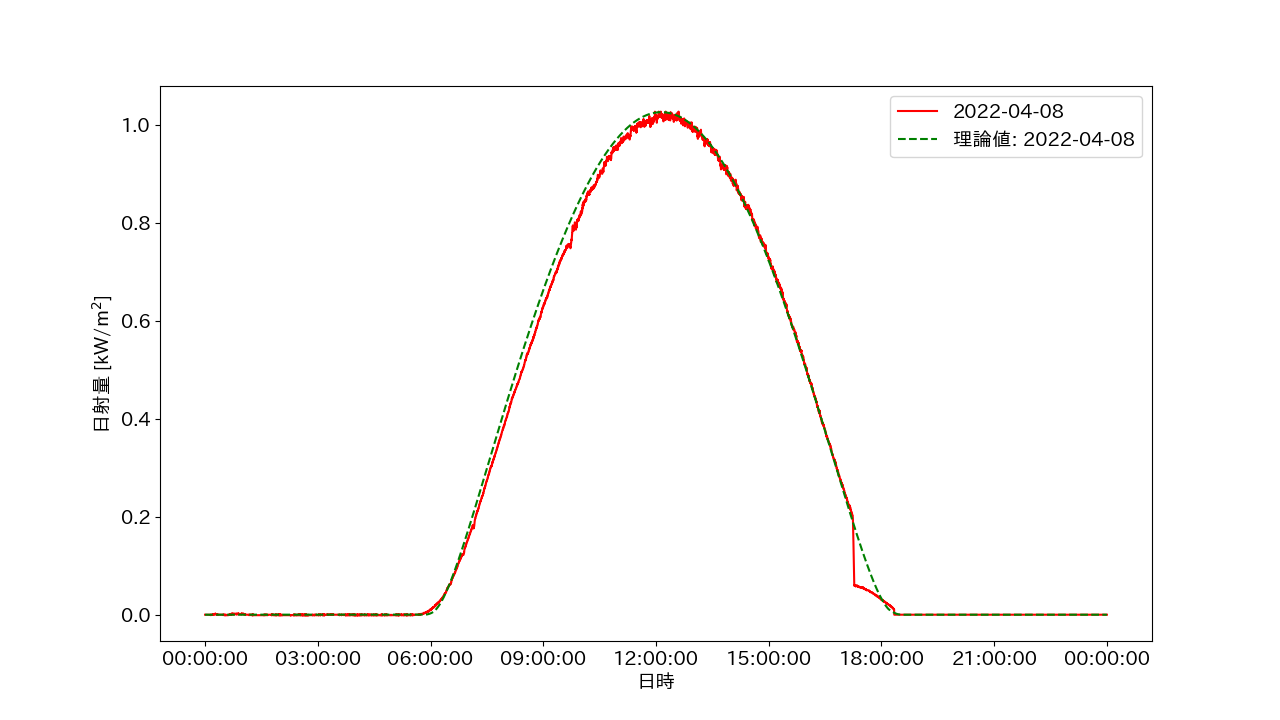
\includegraphics[width=160mm]{real_and_theoretical.png}
    \caption{2022年4月8日の実測データと対応する理論データ}
    \label{p4}
  \end{center}
\end{figure}

このように快晴の日の実測データに対する理論データであれば, 午後の概形は概ね一致する. 午前の概形も一致させるにはpvlibの太陽光パネルが水平面から傾いている角度と, 太陽光パネルが真北から時計回りにどの方向に向いているかを表す角度を調整すればよいが, 月日ごとに再調整する必要がある.

\section{時刻合わせプログラムのアルゴリズムに関する検討}
現在実装されている時刻合わせプログラムでは, 以下のアルゴリズムで実測データと理論データのずれ時間を推定している.

\begin{enumerate}
  \item まず実測データを読み込み, データのサンプリング間隔を1秒ごとの等間隔になるようnumpyのinterp関数を使用して線形補間を行うなど, 前処理を実施する.
  \item 次に実測データのタイムスタンプ情報をPvlibに入力し, 晴天の日における松山Re・再来館の日射量の理論値を計算する.
  \item 最後に, これらの実測データと理論データを用いて相互相関関数を計算し, 最大相関値を持つインデックスを特定する. このインデックスが二つのデータのずれ時間を示し, インデックスに対応する値がラグ時間となる.
\end{enumerate}

例えば, 2022年4月8日の実測データに対してずれ時間を計算した場合, 理論データに対して実測データを165秒進めたときに相互相関が最大となり, ずれ時間の推定結果は-165秒となった. したがって本手法の計算精度は±165秒程度と言える.

時刻合わせプログラムで行う前処理では, 実測データのリサンプリングの他に, 実測データのフィルタリングや正規化などが行われる. この前処理の組み合わせ方によって相互相関によるずれ時間の計算結果が改善するため, 様々な前処理の組み合わせを試みており, それぞれの組み合わせにおける相互相関の計算結果について以下に述べる.

\subsection{指定時間帯外の日射量を0に置き換える実測データの前処理}
2022年4月8日の実測データを観察すると, 日没前に日射量が急激に低下する箇所が存在する.

これは, おそらく松山Re・再来館の周辺にあるマンション等の建物によって太陽光が遮られることが原因と考えられる. このような実測データと理論データで日射量が大きく異なる箇所が相互相関の計算結果に影響を与えていると推測し, そのような箇所を実測データから除去する前処理を実施した.

図 \ref{p6}は, 2022年4月8日の実測データと理論データの日射量が大きく異ならない時間帯に限定してフィルタリングを行い, 相互相関を計算したものである.

このフィルタリングでは, 図 \ref{p6}のように指定時間帯外の実測データと理論データの日射量を0に置き換えている.

\begin{figure}[H]
  \begin{center}
    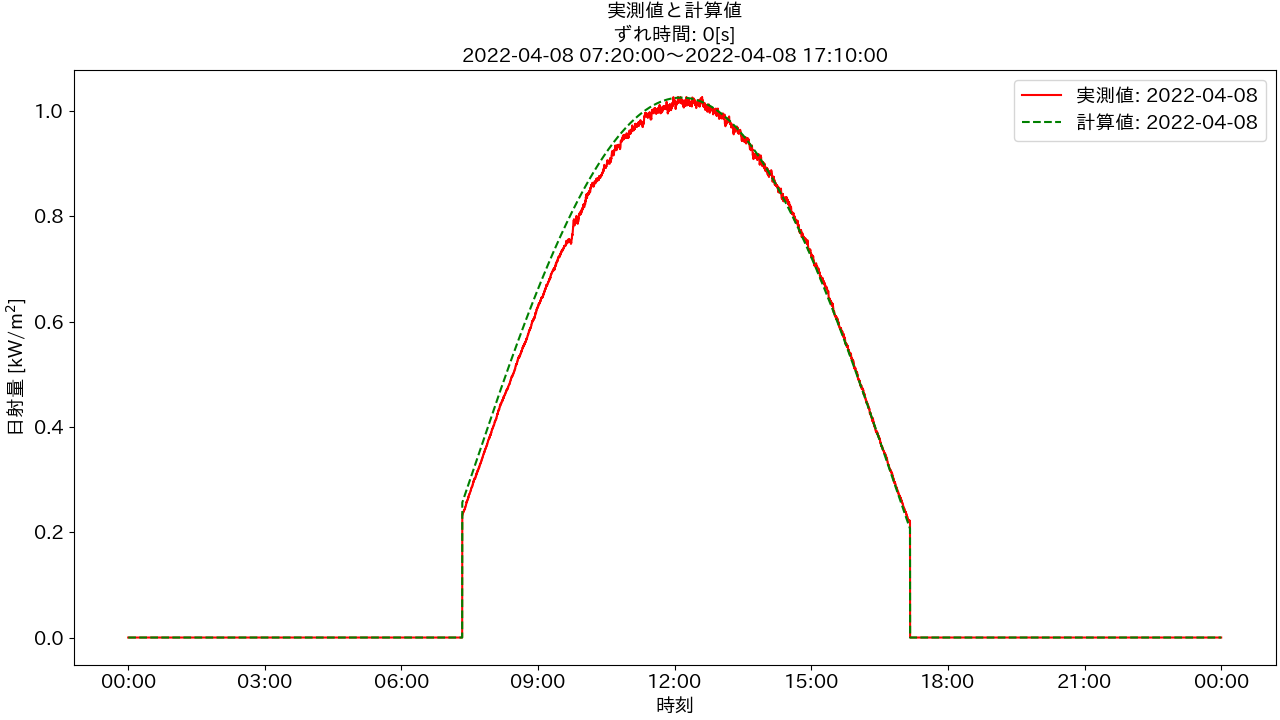
\includegraphics[width=160mm]{2022-04-08_partial_corr.png}
    \caption{フィルタリング後の2022年4月8日の実測データと対応する理論データ}
    \label{p6}
  \end{center}
\end{figure}

相互相関によるずれ時間の推定結果は0秒となり, 一見ずれ時間予測を改善できているように見えるが, 図 \ref{p7}に示すような理論データと概形が大きく異なる実測データを取る日を入力としてずれ時間を推定した際も, 推定結果が0秒となってしまった.

\begin{figure}[H]
  \begin{center}
    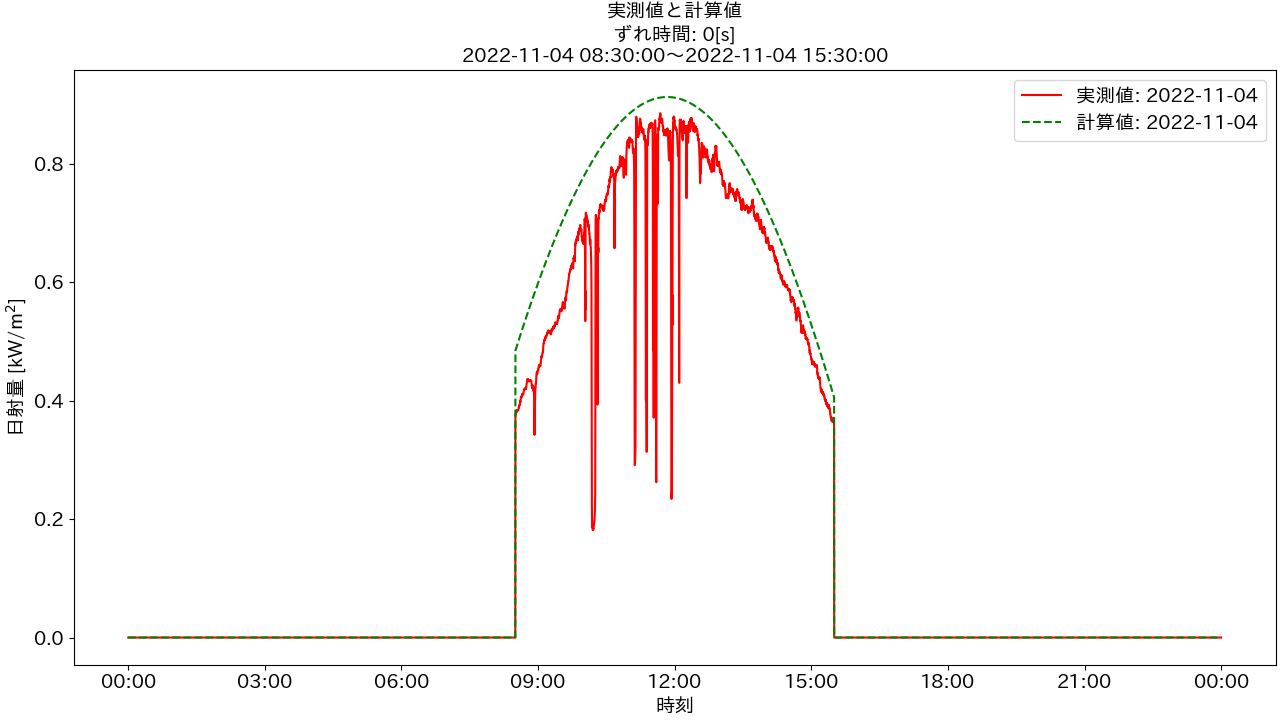
\includegraphics[width=160mm]{2022-11-04_partial_corr.png}
    \caption{フィルタリング後の2022年11月4日の実測データと対応する理論データ}
    \label{p7}
  \end{center}
\end{figure}

このように実測データの概形に関係なく, 推定結果が常に0秒となってしまう原因としては, フィルタリング時に指定時間帯外の日射量を全て0に置き換えたことで, 実測データと理論データの両方において指定時間帯の両端で日射量が0に急激に低下する箇所が現れており, この箇所が相互相関の計算時に強く作用することで, 指定時間帯内の概形に関わらず, ずれ時間の推定結果が常に0秒になってしまうと考えられる.

\subsection{実測データに対する特定の日射量によるフィルタリングおよび日射量の減算}
図 \ref{p7}のように「実測データを, 指定した時間帯外の日射量が0になるように置き換える」という方法では, 指定時間帯の両端において日射量が0へと急激に低下する箇所が相互相関計算に強く影響し, その結果, 相互相関による推定結果が常に0秒になると推測された.

従って, 日射量が0へ急激に低下する箇所を作らずに実測データをフィルタリングする方法として, 図 \ref{p9}に示すように実測データの日射量をしきい値の時にそのしきい値だけ実測データから減算する方法を考案した. ただし減算した時に負になる場合はゼロにしている.

2022/04/08の実測データである図 \ref{p9}では図 \ref{p6}と同様のしきい値である日射量が0.2$\mathrm{kW}/\mathrm{m}^2$以上のデータのみをフィルタリングした結果である.

\begin{figure}[H]
  \begin{center}
    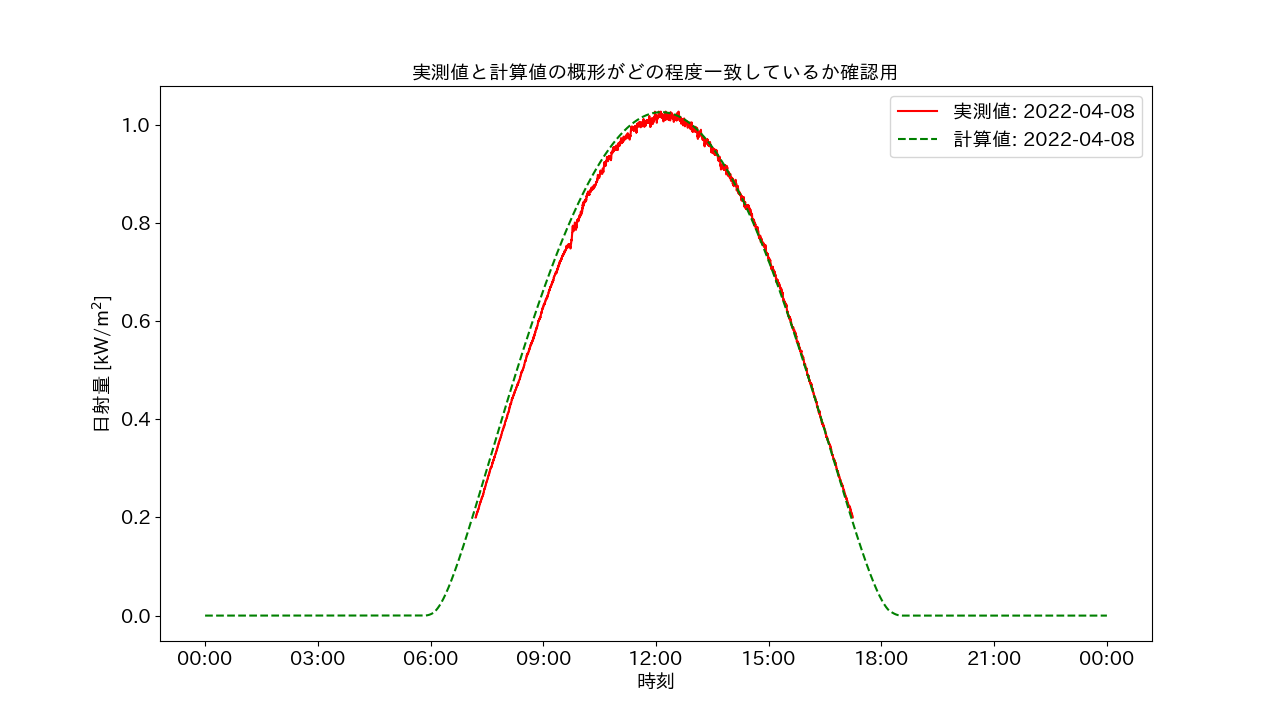
\includegraphics[width=160mm]{2022-04-08_mask_by_q_plot.png}
    \caption{日射量が0.2$\mathrm{kW}/\mathrm{m}^2$以上のみになるようフィルタリングした実測データ}
    \label{p9}
  \end{center}
\end{figure}

そして, 図 \ref{p9}の実測データからフィルタリングの際に指定した日射量の値である0.2だけ減算し, 図 \ref{p10}に示すように下にスライドさせる.

\begin{figure}[H]
  \begin{center}
    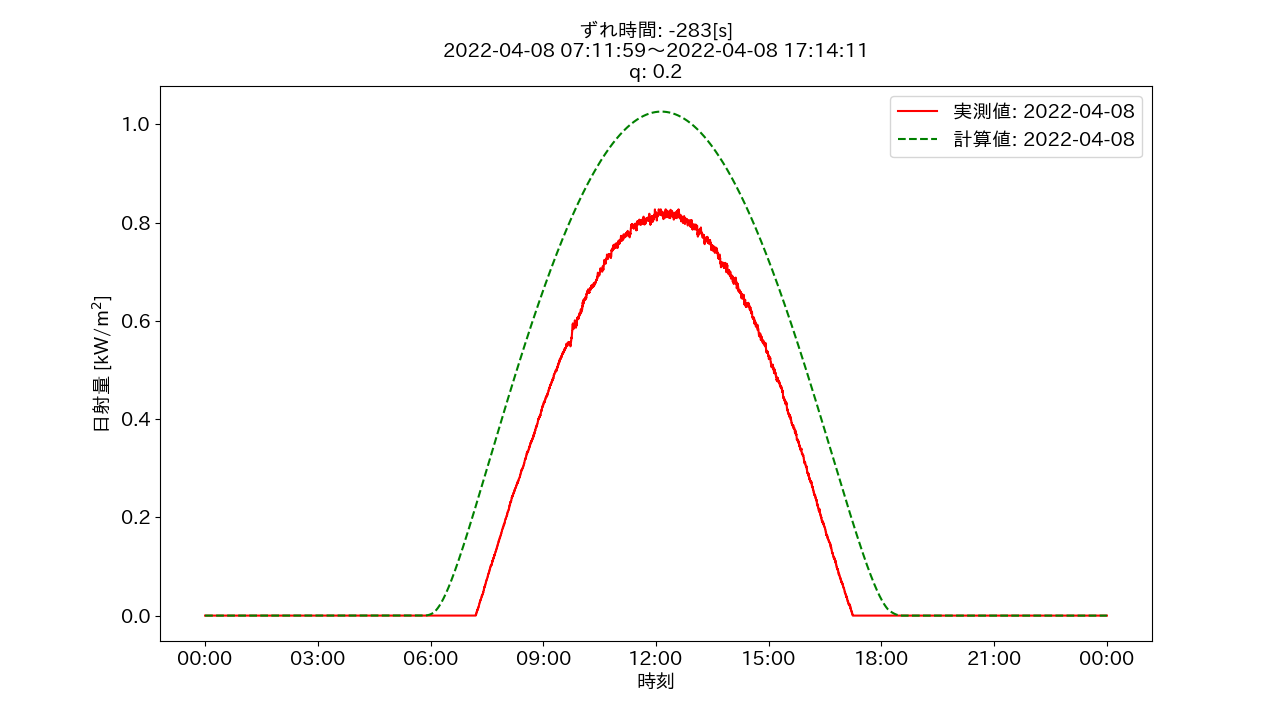
\includegraphics[width=160mm]{2022-04-08_mask_by_q_corr.png}
    \caption{フィルタリングに使用した日射量分, 減算した後の実測データ}
    \label{p10}
  \end{center}
\end{figure}

この方法により, フィルタリングの両端で相互相関計算に強く影響することによって, 推定結果のずれ時間が常に0秒になる問題を回避できることが期待される.

しかしながら, 2022年4月8日のデータにおいては, 相互相関によるずれ時間の推定結果が-283秒となり, 本前処理手法によってずれ時間の推定結果が改善できなかった.

\section{まとめ}
比較的正確に推定できる晴天時における1日分の実測データを入力として時刻合わせプログラムを実行した場合, 推定されたずれ時間は, 期待値よりも165秒程度ずれてることを述べた. 推定ずれ時間を1秒以内にするためには, 今後データの前処理方法あるいは日射量シミュレーションアルゴリズムをさらに改良することが必要がある.

% さらに, 異なる日や天候条件下における実測データを用いて, プログラムの汎用性を評価することも重要であると考えられる. 

\begin{thebibliography}{5}
  \bibitem{1}inoory,"2つの信号間の遅延を推定する",\\ https://qiita.com/inoory/items/3ea2d447f6f1e8c40ffa,参照 Mar 20, 2023.
  \bibitem{2}Sandia National Laboratories and pvlib python Development Team.,"pvlib python — pvlib python 0.9.5 documentation",\\ https://pvlib-python.readthedocs.io/en/stable/,参照 Mar 20, 2023.
\end{thebibliography}

\end{document}